% document type
\documentclass[12pt]{article}

% packages
\usepackage[total={170mm,230mm}]{geometry}
\usepackage[utf8]{inputenc}
\usepackage[T1]{fontenc}
\usepackage[russian]{babel}
\usepackage{graphicx}
\usepackage{amssymb}
\usepackage{amsfonts}
\usepackage{amsmath}
\usepackage{amsthm}
\usepackage{physics}
\usepackage{nicefrac}
\usepackage{cancel}
\usepackage{hyperref}
\usepackage{cmap}

\title{Задание 1}
\author{Козлов Александр}

\begin{document}
	\maketitle
	Сняли анодно\---сеточную характеристику при задерживающем напряжении, при котором видно два максимума анодно\---сеточной характеристики наилучшим образом. Задерживающее напряжение было выбрано $12.1 \pm 0.1\ \text{В}$. Результаты измерений отображены на рисунке \ref{fig:figure1}.
	\begin{figure}[htbp]
		\centering
		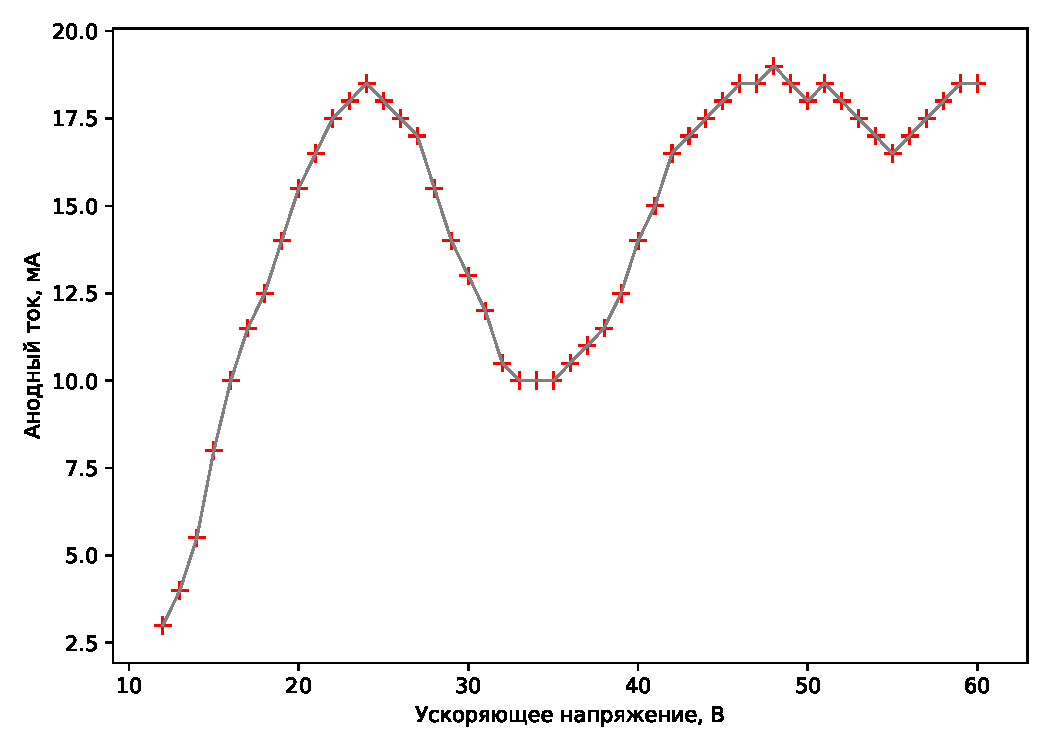
\includegraphics[width=\linewidth]{../plots/1}
		\caption{Анодно-сеточная характеристика при задерживающем напряжении 12.1 В. Видны три локальных максимума при ускоряющем напряжении $24$, $48$ и $51$ $\text{В}$.}
		\label{fig:figure1}
	\end{figure}
	Из положений локальных первых двух локальных максимумов находим резонансный потенциал и разность энергий
	\begin{equation}
		E_1 - E_0 = eV_\text{рез}.
	\end{equation}
	Из наших измерений оказалось, что не важно каким именно образом определять резонансное напряжение. Можно как через напряжение первого локального максимума ($24\ \text{В}$), так и через разность напряжений второго и первого локальных максимумов анодно\---сеточной характеристики ($48 - 24 = 24\ \text{В}$). Таким образом, $V_\text{рез} = 24\ \text{В}$. Откуда следует
	\begin{equation}
		E_1 - E_0 = 24\ \text{эВ} = 3.8\cross10^{-18}\ \text{Дж}.
	\end{equation}
	Не стоит забывать про погрешность измерений (учтём лишь приборные). Поэтому ответом на задание будут следующие численные значения:
	\begin{equation}
		\begin{split}
			&V_\text{рез} = 24.0\pm0.5\ \text{В};\\
			&E_1 - E_0 = 24.0\pm0.5\ \text{эВ} = (3.85\pm0.08)\cross10^{-18}\ \text{Дж}.
		\end{split}
	\end{equation}
\end{document}